% Options for packages loaded elsewhere
\PassOptionsToPackage{unicode}{hyperref}
\PassOptionsToPackage{hyphens}{url}
%
\documentclass[
  ignorenonframetext,
]{beamer}
\usepackage{pgfpages}
\setbeamertemplate{caption}[numbered]
\setbeamertemplate{caption label separator}{: }
\setbeamercolor{caption name}{fg=normal text.fg}
\beamertemplatenavigationsymbolsempty
% Prevent slide breaks in the middle of a paragraph
\widowpenalties 1 10000
\raggedbottom
\setbeamertemplate{part page}{
  \centering
  \begin{beamercolorbox}[sep=16pt,center]{part title}
    \usebeamerfont{part title}\insertpart\par
  \end{beamercolorbox}
}
\setbeamertemplate{section page}{
  \centering
  \begin{beamercolorbox}[sep=12pt,center]{part title}
    \usebeamerfont{section title}\insertsection\par
  \end{beamercolorbox}
}
\setbeamertemplate{subsection page}{
  \centering
  \begin{beamercolorbox}[sep=8pt,center]{part title}
    \usebeamerfont{subsection title}\insertsubsection\par
  \end{beamercolorbox}
}
\AtBeginPart{
  \frame{\partpage}
}
\AtBeginSection{
  \ifbibliography
  \else
    \frame{\sectionpage}
  \fi
}
\AtBeginSubsection{
  \frame{\subsectionpage}
}
\usepackage{amsmath,amssymb}
\usepackage{iftex}
\ifPDFTeX
  \usepackage[T1]{fontenc}
  \usepackage[utf8]{inputenc}
  \usepackage{textcomp} % provide euro and other symbols
\else % if luatex or xetex
  \usepackage{unicode-math} % this also loads fontspec
  \defaultfontfeatures{Scale=MatchLowercase}
  \defaultfontfeatures[\rmfamily]{Ligatures=TeX,Scale=1}
\fi
\usepackage{lmodern}
\usetheme[]{Frankfurt}
\ifPDFTeX\else
  % xetex/luatex font selection
\fi
% Use upquote if available, for straight quotes in verbatim environments
\IfFileExists{upquote.sty}{\usepackage{upquote}}{}
\IfFileExists{microtype.sty}{% use microtype if available
  \usepackage[]{microtype}
  \UseMicrotypeSet[protrusion]{basicmath} % disable protrusion for tt fonts
}{}
\makeatletter
\@ifundefined{KOMAClassName}{% if non-KOMA class
  \IfFileExists{parskip.sty}{%
    \usepackage{parskip}
  }{% else
    \setlength{\parindent}{0pt}
    \setlength{\parskip}{6pt plus 2pt minus 1pt}}
}{% if KOMA class
  \KOMAoptions{parskip=half}}
\makeatother
\usepackage{xcolor}
\newif\ifbibliography
\usepackage{color}
\usepackage{fancyvrb}
\newcommand{\VerbBar}{|}
\newcommand{\VERB}{\Verb[commandchars=\\\{\}]}
\DefineVerbatimEnvironment{Highlighting}{Verbatim}{commandchars=\\\{\}}
% Add ',fontsize=\small' for more characters per line
\usepackage{framed}
\definecolor{shadecolor}{RGB}{248,248,248}
\newenvironment{Shaded}{\begin{snugshade}}{\end{snugshade}}
\newcommand{\AlertTok}[1]{\textcolor[rgb]{0.94,0.16,0.16}{#1}}
\newcommand{\AnnotationTok}[1]{\textcolor[rgb]{0.56,0.35,0.01}{\textbf{\textit{#1}}}}
\newcommand{\AttributeTok}[1]{\textcolor[rgb]{0.13,0.29,0.53}{#1}}
\newcommand{\BaseNTok}[1]{\textcolor[rgb]{0.00,0.00,0.81}{#1}}
\newcommand{\BuiltInTok}[1]{#1}
\newcommand{\CharTok}[1]{\textcolor[rgb]{0.31,0.60,0.02}{#1}}
\newcommand{\CommentTok}[1]{\textcolor[rgb]{0.56,0.35,0.01}{\textit{#1}}}
\newcommand{\CommentVarTok}[1]{\textcolor[rgb]{0.56,0.35,0.01}{\textbf{\textit{#1}}}}
\newcommand{\ConstantTok}[1]{\textcolor[rgb]{0.56,0.35,0.01}{#1}}
\newcommand{\ControlFlowTok}[1]{\textcolor[rgb]{0.13,0.29,0.53}{\textbf{#1}}}
\newcommand{\DataTypeTok}[1]{\textcolor[rgb]{0.13,0.29,0.53}{#1}}
\newcommand{\DecValTok}[1]{\textcolor[rgb]{0.00,0.00,0.81}{#1}}
\newcommand{\DocumentationTok}[1]{\textcolor[rgb]{0.56,0.35,0.01}{\textbf{\textit{#1}}}}
\newcommand{\ErrorTok}[1]{\textcolor[rgb]{0.64,0.00,0.00}{\textbf{#1}}}
\newcommand{\ExtensionTok}[1]{#1}
\newcommand{\FloatTok}[1]{\textcolor[rgb]{0.00,0.00,0.81}{#1}}
\newcommand{\FunctionTok}[1]{\textcolor[rgb]{0.13,0.29,0.53}{\textbf{#1}}}
\newcommand{\ImportTok}[1]{#1}
\newcommand{\InformationTok}[1]{\textcolor[rgb]{0.56,0.35,0.01}{\textbf{\textit{#1}}}}
\newcommand{\KeywordTok}[1]{\textcolor[rgb]{0.13,0.29,0.53}{\textbf{#1}}}
\newcommand{\NormalTok}[1]{#1}
\newcommand{\OperatorTok}[1]{\textcolor[rgb]{0.81,0.36,0.00}{\textbf{#1}}}
\newcommand{\OtherTok}[1]{\textcolor[rgb]{0.56,0.35,0.01}{#1}}
\newcommand{\PreprocessorTok}[1]{\textcolor[rgb]{0.56,0.35,0.01}{\textit{#1}}}
\newcommand{\RegionMarkerTok}[1]{#1}
\newcommand{\SpecialCharTok}[1]{\textcolor[rgb]{0.81,0.36,0.00}{\textbf{#1}}}
\newcommand{\SpecialStringTok}[1]{\textcolor[rgb]{0.31,0.60,0.02}{#1}}
\newcommand{\StringTok}[1]{\textcolor[rgb]{0.31,0.60,0.02}{#1}}
\newcommand{\VariableTok}[1]{\textcolor[rgb]{0.00,0.00,0.00}{#1}}
\newcommand{\VerbatimStringTok}[1]{\textcolor[rgb]{0.31,0.60,0.02}{#1}}
\newcommand{\WarningTok}[1]{\textcolor[rgb]{0.56,0.35,0.01}{\textbf{\textit{#1}}}}
\setlength{\emergencystretch}{3em} % prevent overfull lines
\providecommand{\tightlist}{%
  \setlength{\itemsep}{0pt}\setlength{\parskip}{0pt}}
\setcounter{secnumdepth}{-\maxdimen} % remove section numbering
\usepackage{dcolumn}
\usepackage{longtable,booktabs}
\makeatletter\def\fnum@table{\usebeamercolor{caption name}\usebeamerfont*{caption name}\tablename~\thetable}\makeatother
\usepackage{fvextra}
\DefineVerbatimEnvironment{Highlighting}{Verbatim}{ breaksymbolleft={}, showspaces = false, showtabs = false, breaklines, commandchars=\\\{\} }
\ifLuaTeX
  \usepackage{selnolig}  % disable illegal ligatures
\fi
\IfFileExists{bookmark.sty}{\usepackage{bookmark}}{\usepackage{hyperref}}
\IfFileExists{xurl.sty}{\usepackage{xurl}}{} % add URL line breaks if available
\urlstyle{same}
\hypersetup{
  pdftitle={Beyond Normalization: Incorporating Scale Uncertainty in ALDEx2},
  pdfauthor={Michelle Nixon},
  hidelinks,
  pdfcreator={LaTeX via pandoc}}

\title{Beyond Normalization: Incorporating Scale Uncertainty in ALDEx2}
\author{Michelle Nixon}
\date{May 13, 2024}
\institute{The Silverman Lab\\
College of Information Sciences and Technology\\
Penn State University}

\begin{document}
\frame{\titlepage}

\begin{frame}{Recap: Sequencing depth can confound conclusions.}
\protect\hypertarget{recap-sequencing-depth-can-confound-conclusions.}{}
\begin{table}[h!]
\centering
\begin{tabular}{|r|c c c| c|}
\hline
\textcolor{gray}{Observed data (Y)} & Sample 1 & Sample 2 & Sample 3  &\\
\hline
Condition & Pre & Pre & Post & \textcolor{gray}{Conclusion}\\
\hline
Entity 1 & 5 & 10 & 100 & \textcolor{gray}{Increase}\\
Entity 2 & 10 & 25 & 3 & \textcolor{gray}{Decrease}\\
Entity 3 & 0 & 1 & 8 & \textcolor{gray}{Increase}\\
Entity 4 & 0 & 0 & 19 &\textcolor{gray}{Increase}\\
\hline
\textcolor{gray}{Sequencing Depth} & \textcolor{gray}{15} & \textcolor{gray}{36} & \textcolor{gray}{130} &\\
\hline
\end{tabular}
\end{table}
\end{frame}

\begin{frame}{This can mislead analyses.}
\protect\hypertarget{this-can-mislead-analyses.}{}
\begin{table}[h!]
\centering
\begin{tabular}{|r|c c c| c|}
\hline
\textcolor{gray}{System data (W)} & Sample 1 & Sample 2 & Sample 3  & \\
\hline
Condition & Pre & Pre & Post & \textcolor{gray}{Conclusion}\\
\hline
Entity 1 & 227 & 351 & 154 & \textcolor{gray}{Decrease}\\
Entity 2 & 684 & 891 & 3 & \textcolor{gray}{Decrease}\\
Entity 3 & 48 & 32 & 15 & \textcolor{gray}{Decrease}\\
Entity 4 & 43 & 39  & 27 &\textcolor{gray}{Decrease}\\
\hline
\textcolor{gray}{Scale ($W^\perp$)} & \textcolor{gray}{1,002} & \textcolor{gray}{1,313} & \textcolor{gray}{200} &\\
\hline
\end{tabular}
\end{table}
\end{frame}

\begin{frame}{\ldots{} and lead to unacknowledged bias.}
\protect\hypertarget{and-lead-to-unacknowledged-bias.}{}
\begin{figure}
  \centering
  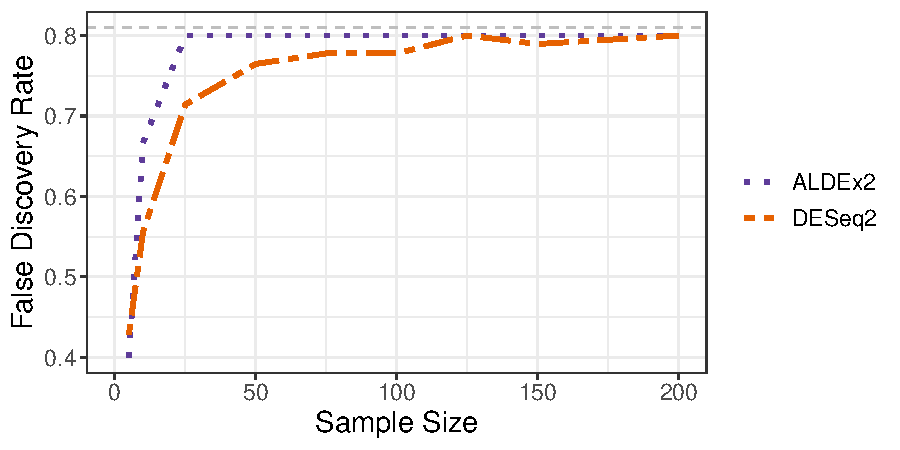
\includegraphics[width=4.5in]{figures/unacknowledged_bias.pdf}
\end{figure}
\end{frame}

\hypertarget{problem-set-up}{%
\section{Problem Set-Up}\label{problem-set-up}}

\begin{frame}{Observed Data as a Sample from the System}
\protect\hypertarget{observed-data-as-a-sample-from-the-system}{}
\begin{figure}
  \centering
  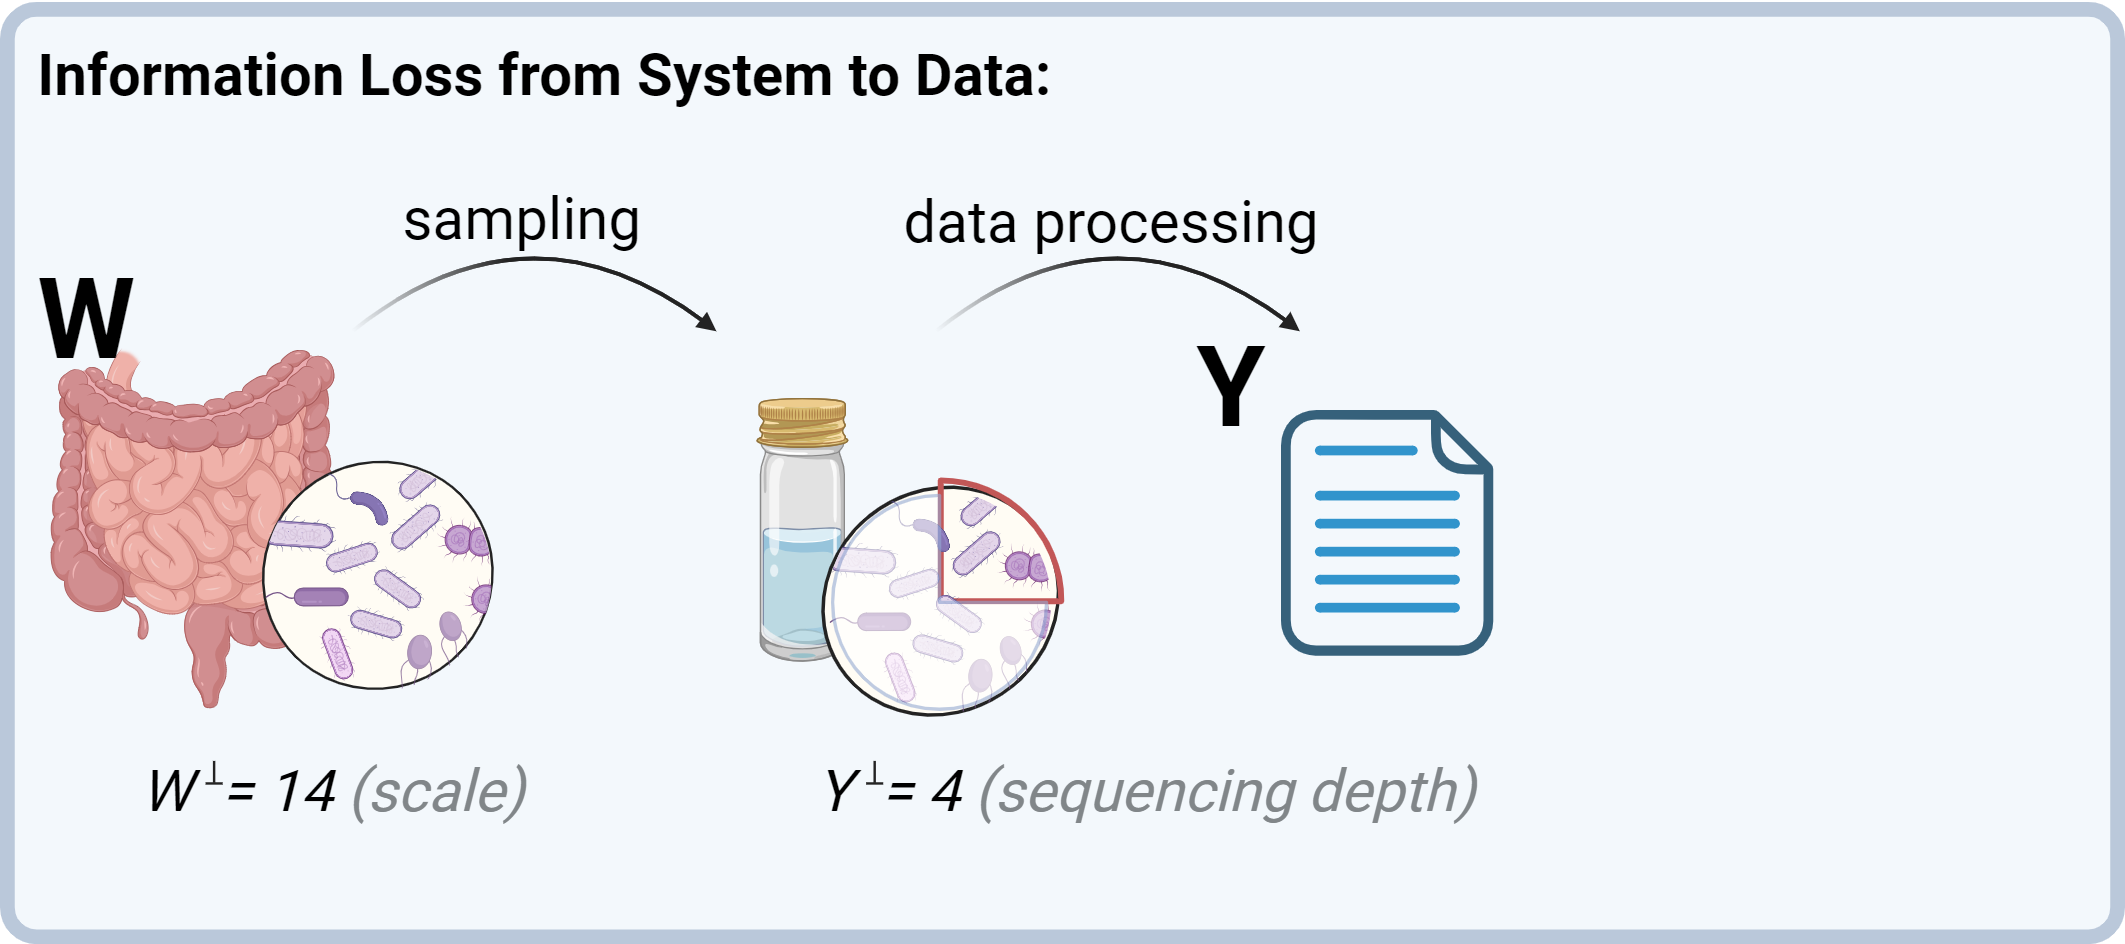
\includegraphics[width=4.5in]{figures/intro-fig-first.png}
\end{figure}
\end{frame}

\begin{frame}{Observed Data as a Sample from the System}
\protect\hypertarget{observed-data-as-a-sample-from-the-system-1}{}
\begin{figure}
  \centering
  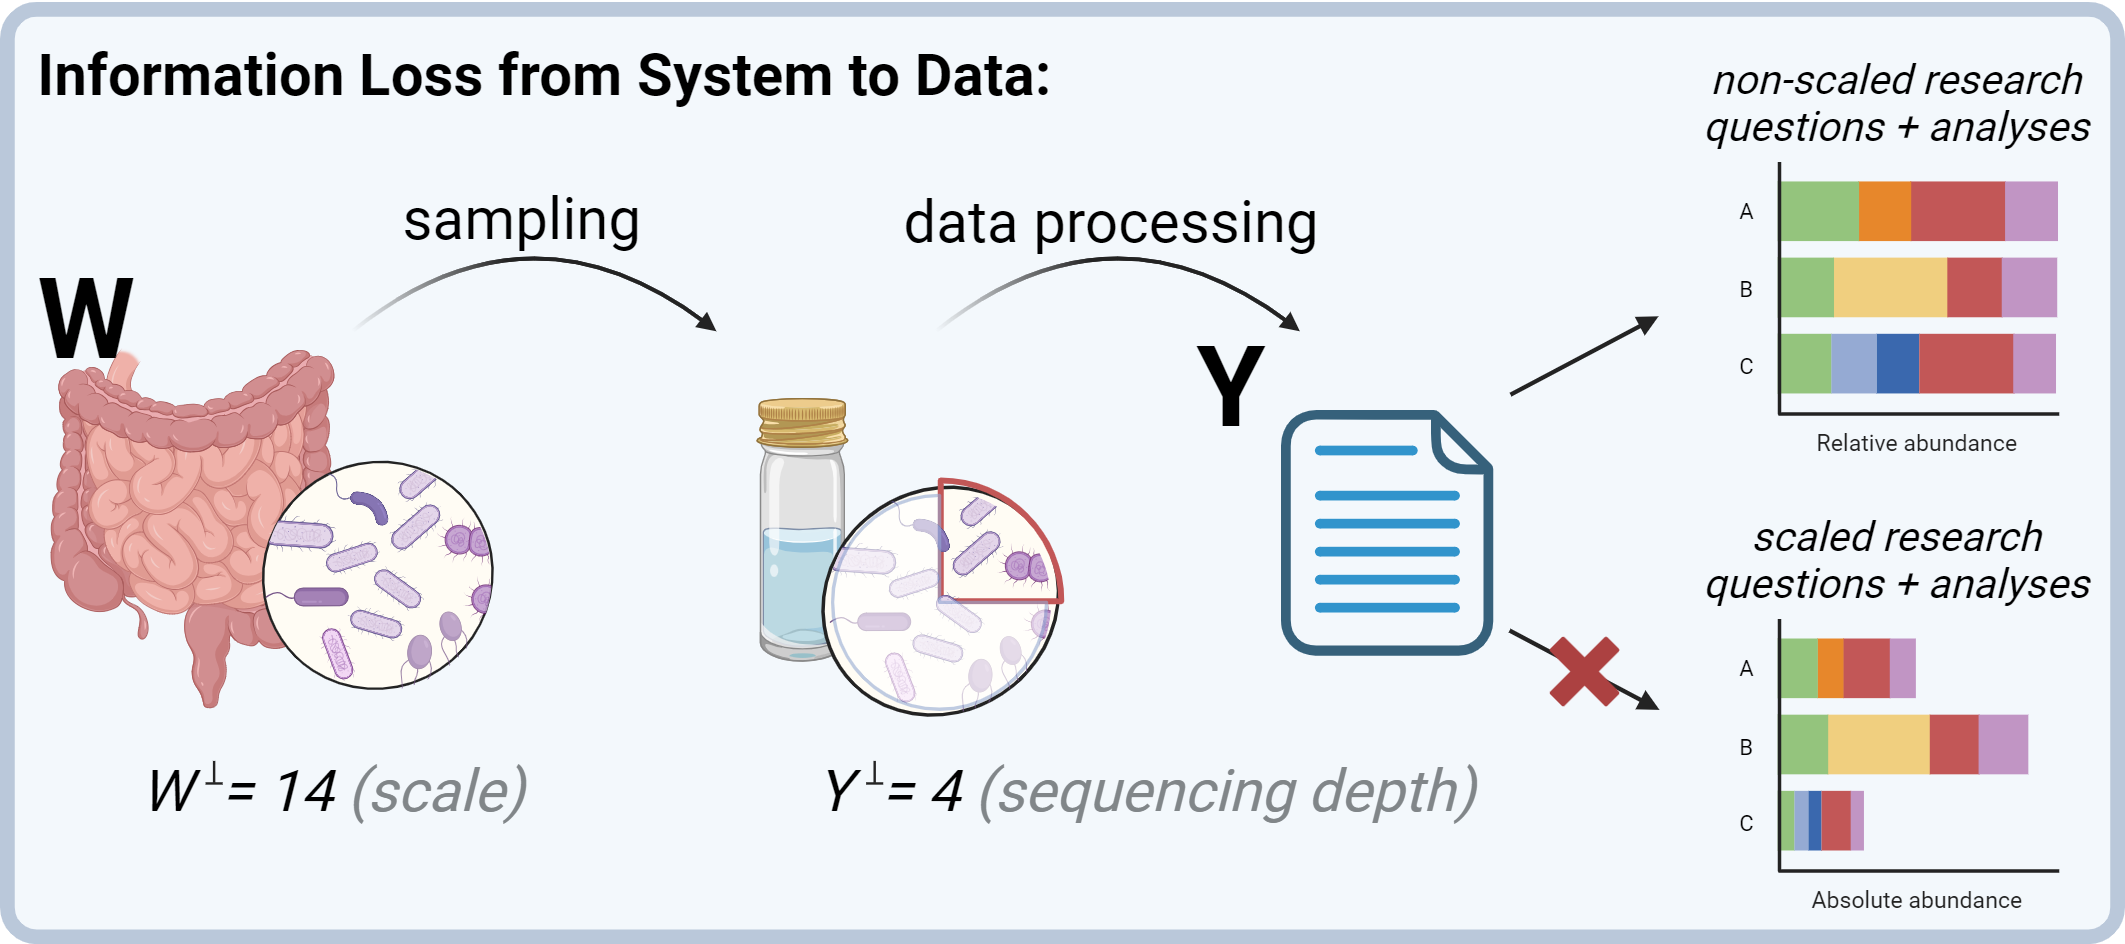
\includegraphics[width=4.5in]{figures/intro-fig-full.png}
\end{figure}
\end{frame}

\begin{frame}{Notation}
\protect\hypertarget{notation}{}
\begin{itemize}
\tightlist
\item
  \(\mathbf{Y}\): a measurement of the underlying system \(\mathbf{W}\).
\end{itemize}

\[\mathbf{W}_{dn} = \underbrace{\mathbf{W}_{dn}^\parallel}_{\text{composition}} \times  \underbrace{W_n^\perp}_{\text{scale}}\]
\pause

\begin{itemize}
\item
  \textbf{Composition:}
  \(\mathbf{W}_{dn}^\parallel = \frac{\mathbf{W}_{dn}}{\sum_{d=1}^D \mathbf{W}_{dn}}\)
\item
  \textbf{Scale:} \(W_n^\perp = \sum_{d=1}^D \mathbf{W}_{dn}\)
\end{itemize}
\end{frame}

\begin{frame}{Example: Notation}
\protect\hypertarget{example-notation}{}
\begin{table}[h!]
\centering
\begin{tabular}{|r|c c c| }
\hline
\textcolor{gray}{System data ($W^\parallel$)} & Sample 1 & Sample 2 & Sample 3\\
\hline
Condition & Pre & Pre & Post\\
\hline
Entity 1 & 0.27 & 0.27 & 0.77 \\
Entity 2 & 0.68 & 0.68 & 0.02 \\
Entity 3 & 0.05 & 0.02 & 0.08 \\
Entity 4 & 0.04 & 0.03  & 0.13 \\
\hline
\end{tabular}
\end{table}

\begin{table}[h!]
\centering
\begin{tabular}{|r|c c c| }
\hline
 & Sample 1 & Sample 2 & Sample 3\\
\hline
Condition & Pre & Pre & Post\\
\hline
\textcolor{gray}{Scale ($W^\perp$)} & \textcolor{gray}{1,002} & \textcolor{gray}{1,313} & \textcolor{gray}{200}\\
\hline
\end{tabular}
\end{table}
\end{frame}

\begin{frame}{Differential Abundance/Expression Analysis}
\protect\hypertarget{differential-abundanceexpression-analysis}{}
\begin{itemize}
\tightlist
\item
  \textbf{Research Question:} How do entities (e.g., taxa or genes)
  change between conditions?
\end{itemize}

\vspace{.075in}

\begin{itemize}
\tightlist
\item
  \(\boldsymbol{\theta}\): what we want to estimate.
  \textcolor{white}{(Log Fold Change)}
\end{itemize}

\vspace{.075in}

\begin{equation*}
\theta_d = \text{mean}_{\text{case}}(\log \mathbf{W}_{dn}) - \text{mean}_{\text{control}}(\log \mathbf{W}_{dn})
\end{equation*}
\end{frame}

\begin{frame}{The Original ALDEx2 Model}
\protect\hypertarget{the-original-aldex2-model}{}
\textbf{Step 1: Model Sampling Uncertainty} \begin{align*}
\mathbf{Y}_{\cdot n} &\sim \text{Multinomial}(\mathbf{W}_{\cdot n}^\parallel)\\
\mathbf{W}_{\cdot n}^\parallel &\sim \text{Dirichlet}(\alpha)
\end{align*}

\textbf{Step 2: Centered Log-Ratio Transformation} \begin{equation*}
\log \mathbf{W}_{\cdot n} = \left[\log \mathbf{W}_{1n}^\parallel - \text{mean}(\log \mathbf{W}_{\cdot n}^\parallel), ..., \log \mathbf{W}_{Dn}^\parallel - \text{mean}(\log \mathbf{W}_{\cdot n}^\parallel) \right]
\end{equation*}

\textbf{Step 3: Calculate LFCs and Test if Different from Zero.}
\begin{equation*}
\theta_d = \text{mean}_{\text{case}}(\log \mathbf{W}_{dn}) - \text{mean}_{\text{control}}(\log \mathbf{W}_{dn})
\end{equation*}
\end{frame}

\begin{frame}{Implied Assumptions about Scale}
\protect\hypertarget{implied-assumptions-about-scale}{}
\textcolor{gray}{\textbf{Step 1: Model Sampling Uncertainty}}
\begin{align*}
\textcolor{gray}{\mathbf{Y}_{\cdot n}} &\textcolor{gray}{\sim \text{Multinomial}(\mathbf{W}_{\cdot n}^\parallel)}\\
\textcolor{gray}{\mathbf{W}_{\cdot n}^\parallel} &\textcolor{gray}{\sim \text{Dirichlet}(\alpha)}
\end{align*}

\textbf{Step 2: Centered Log-Ratio Transformation} \begin{equation*}
\log \mathbf{W}_{\cdot n} = \left[\log \mathbf{W}_{1n}^\parallel - \text{mean}(\log \mathbf{W}_{\cdot n}^\parallel), ..., \log \mathbf{W}_{Dn}^\parallel - \text{mean}(\log \mathbf{W}_{\cdot n}^\parallel) \right]
\end{equation*}

\textcolor{gray}{\textbf{Step 3: Calculate LFCs and Test if Different from Zero.}
\begin{equation*}
\theta_d = \text{mean}_{\text{case}}(\log \mathbf{W}_{dn}) - \text{mean}_{\text{control}}(\log \mathbf{W}_{dn})
\end{equation*}}
\end{frame}

\begin{frame}{Implied Assumptions about Scale, cont.}
\protect\hypertarget{implied-assumptions-about-scale-cont.}{}
Since
\(\log \mathbf{W}_{dn} = \log \mathbf{W}_{dn}^\parallel + \log W_n^\perp\),
the CLR normalization implies:

\begin{align*}
\color{gray}{\log W_{dn}} &= \color{gray}{\log \mathbf{W}_{dn}^\parallel - \text{mean}(\log \mathbf{W}_{\cdot n}^\parallel)}\\
\log W_n^\perp &= -\text{mean}(\log \mathbf{W}_{\cdot n}^\parallel).
\end{align*}

\vspace{.25in}

\textcolor{gray}{What happens when this is wrong?}
\end{frame}

\begin{frame}{Unacknowledged bias!}
\protect\hypertarget{unacknowledged-bias}{}
\begin{figure}
  \centering
  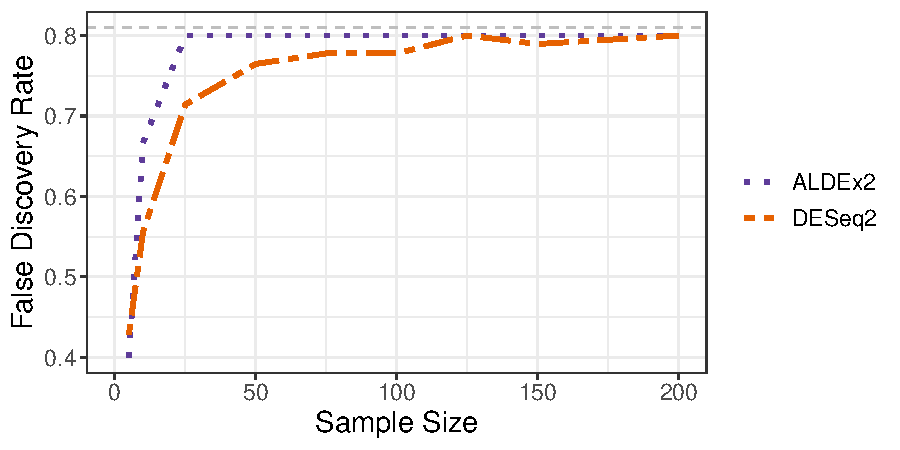
\includegraphics[width=4.5in]{figures/unacknowledged_bias.pdf}
\end{figure}
\end{frame}

\begin{frame}{Adding Uncertainty in Scale can Help.}
\protect\hypertarget{adding-uncertainty-in-scale-can-help.}{}
\begin{figure}
  \centering
  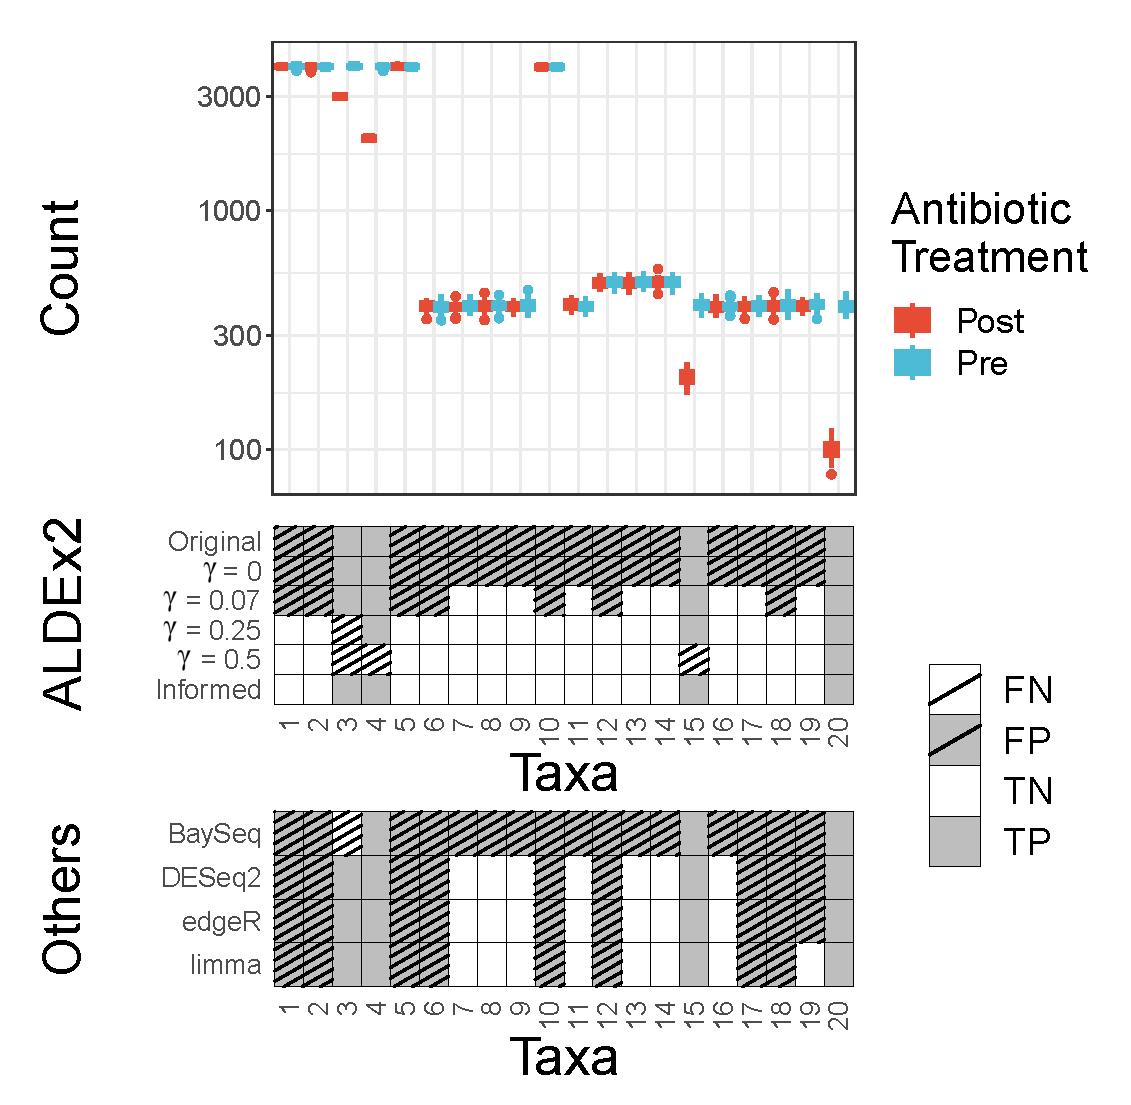
\includegraphics[width=3.25in]{figures/sim-res.pdf}
\end{figure}
\end{frame}

\hypertarget{scale-reliant-inference}{%
\section{Scale Reliant Inference}\label{scale-reliant-inference}}

\begin{frame}{Scale Reliant Inference: The Basics}
\protect\hypertarget{scale-reliant-inference-the-basics}{}
\begin{itemize}
\item
  \textbf{The CoDA perspective:} Research questions that depend on
  \(W^\perp\) (scale) cannot be answered rigorously.
\item
  \textbf{The Normalization perspective:} Research questions that depend
  on \(W^\perp\) (scale) can be answered after normalization.
\item
  Who is right?
\end{itemize}

\pause

\begin{itemize}
\item
  \textbf{The CoDA perspective:} Rigourous, but scientifically limiting.
\item
  \textbf{The Normalization perspective:} Practical, but unacknowledged
  bias.
\end{itemize}
\end{frame}

\begin{frame}{Scale Reliant Inference: The Basics}
\protect\hypertarget{scale-reliant-inference-the-basics-1}{}
\begin{itemize}
\tightlist
\item
  For LFCs, \(\theta\) depends on \(W^\perp\):
\end{itemize}

\begin{align*}
\theta_d &= \text{mean}_{\text{case}}(\log \mathbf{W}_{dn}) - \text{mean}_{\text{control}}(\log \mathbf{W}_{dn})\\
&= ... \\
&= \underbrace{\text{mean}_{\text{case}}(\log \mathbf{W}_{dn}^\parallel) - \text{mean}_{\text{control}}(\log \mathbf{W}_{dn}^\parallel)}_{\theta^\parallel}\\
& \, \, \, \, \, \, + \underbrace{\text{mean}_{\text{case}}(\log W_{n}^\perp) - \text{mean}_{\text{control}}(\log W_{n}^\perp)}_{\theta^\perp}\\
\end{align*}
\end{frame}

\begin{frame}{Scale Reliant Inference: Theory Intro}
\protect\hypertarget{scale-reliant-inference-theory-intro}{}
Recall for LFCs: \begin{align*}
\theta_d &= \text{mean}_{\text{case}}(\log \mathbf{W}_{dn} ) - \text{mean}_{\text{control}}(\log \mathbf{W}_{dn} )\\
&= \theta^\parallel + \theta^\perp
\end{align*}

\begin{itemize}
\tightlist
\item
  What can we say about \(\theta\) from \(\theta^\parallel\) alone?
\end{itemize}

\pause

\begin{itemize}
\item
  Statistical perspective: \(\theta\) is not identifiable without
  \(\theta^\perp\).
\item
  Practical issues: unbiased estimators, calibrated confidence sets, and
  type-I error control \textbf{NOT} possible!
\item
  See Nixon et al.~(2023) for details.
\end{itemize}
\end{frame}

\begin{frame}{\(\theta^\perp\): The Missing Piece}
\protect\hypertarget{thetaperp-the-missing-piece}{}
\textcolor{gray}{\begin{equation*}
\theta^\perp = \text{mean}_{\text{case}}(\log W_{n}^\perp) - \text{mean}_{\text{control}}(\log W_{n}^\perp)
\end{equation*}}

\vspace{.1in}
\pause

\begin{itemize}
\item
  The change in scales between conditions matters for estimating LFCs.
\item
  The scale only needs to be known up to a constant (see Nixon et. al
  (2023)).
\end{itemize}

\pause

\begin{itemize}
\tightlist
\item
  Each normalization implies a value of \(\theta^\perp\)
  \textcolor{gray}{(e.g., CLR):}
\end{itemize}

\textcolor{gray}{\begin{equation*}
\theta^\perp_{\text{CLR}} = \text{mean}_{\text{case}}(- \log \text{GM}( \mathbf{W}_{\cdot n}^\parallel)) - \text{mean}_{\text{control}}(- \log \text{GM}( \mathbf{W}_{\cdot n}^\parallel)) 
\end{equation*}}
\end{frame}

\begin{frame}{Scale Simulation Random Variables}
\protect\hypertarget{scale-simulation-random-variables}{}
\textbf{Goal:} Estimate \(\theta = f(\mathbf{W}^\parallel, W^\perp)\).

\vspace{.1in}

\begin{enumerate}
\item
  Draw samples of \(\mathbf{W}^{\parallel}\) from a measurement model
  \textcolor{gray}{(can depend on $Y$)}.
\item
  Draw samples of \(W^{\perp}\) from a scale model
  \textcolor{gray}{(can depend on $\mathbf{W}^\parallel$)}.
\item
  Estimate samples of \(\theta = f(\mathbf{W}^\parallel, W^\perp)\).
\end{enumerate}
\end{frame}

\begin{frame}{Comparison to ALDEx2}
\protect\hypertarget{comparison-to-aldex2}{}
\begin{block}{The ALDEx2 Model}

\textbf{Step 1: Model Sampling Uncertainty}
\begin{align*}
\mathbf{Y}_{\cdot n} &\sim \text{Multinomial}(\mathbf{W}_{\cdot n}^\parallel)\\
\mathbf{W}_{\cdot n}^\parallel &\sim \text{Dirichlet}(\alpha)
\end{align*}

\textbf{Step 2: Centered Log-Ratio Transformation}
\begin{equation*}
\log \mathbf{W}_{\cdot n} = \left[\log \mathbf{W}_{1n}^\parallel - \text{mean}(\log \mathbf{W}_{\cdot n}^\parallel), ..., \log \mathbf{W}_{Dn}^\parallel - \text{mean}(\log \mathbf{W}_{\cdot n}^\parallel) \right]
\end{equation*}

\textbf{Step 3: Calculate LFCs and Test if Different from Zero.}

\end{block}
\end{frame}

\begin{frame}{The Original Scale Model}
\protect\hypertarget{the-original-scale-model}{}
\begin{figure}
  \centering
  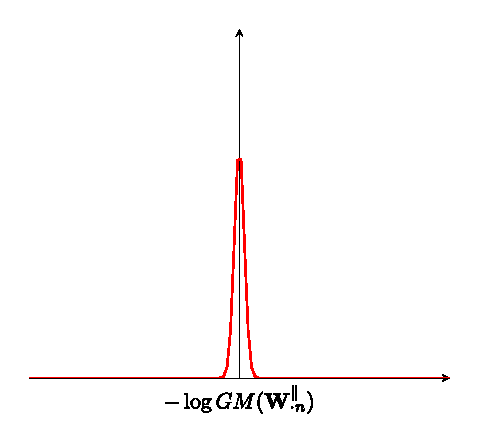
\includegraphics[width=3in]{figures/scale-model-figure-1.pdf}
\end{figure}
\end{frame}

\begin{frame}{Extending the Original Scale Model}
\protect\hypertarget{extending-the-original-scale-model}{}
\begin{figure}
  \centering
  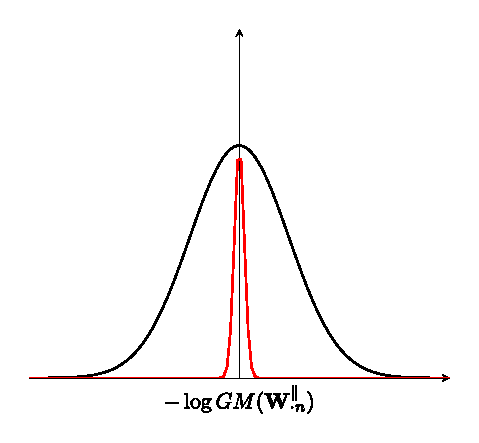
\includegraphics[width=3in]{figures/scale-model-figure-2.pdf}
\end{figure}
\end{frame}

\begin{frame}{ALDEx2 as an SSRV}
\protect\hypertarget{aldex2-as-an-ssrv}{}
\textcolor{gray}{\textbf{Step 1: Model Sampling Uncertainty}}
\textcolor{gray}{\begin{align*}
\mathbf{Y}_{\cdot n} &\sim \text{Multinomial}(\mathbf{W}_{\cdot n}^\parallel)\\
\mathbf{W}_{\cdot n}^\parallel &\sim \text{Dirichlet}(\alpha)
\end{align*}}

\textbf{Step 2: Draw Samples from a Scale Model} \begin{align*}
\log W_{n}^\perp &=- \text{mean}(\log \mathbf{W}_{\cdot n}^\parallel) + \epsilon, \, \epsilon \sim N(0,\gamma^2)\\
\log \mathbf{W}_{\cdot n} &= \log \mathbf{W}_{\cdot n}^\parallel + \log W_{n}^\perp
\end{align*}

\textcolor{gray}{\textbf{Step 3: Calculate LFCs and Test if Different from Zero.}}
\textcolor{gray}{\begin{equation*}
\theta_d = \text{mean}_{\text{case}}(\log \mathbf{W}_{dn}) - \text{mean}_{\text{control}}(\log \mathbf{W}_{dn})
  \end{equation*}}
\end{frame}

\begin{frame}{Benefits of Moving Past Normalizations to Scale}
\protect\hypertarget{benefits-of-moving-past-normalizations-to-scale}{}
\begin{figure}
  \centering
  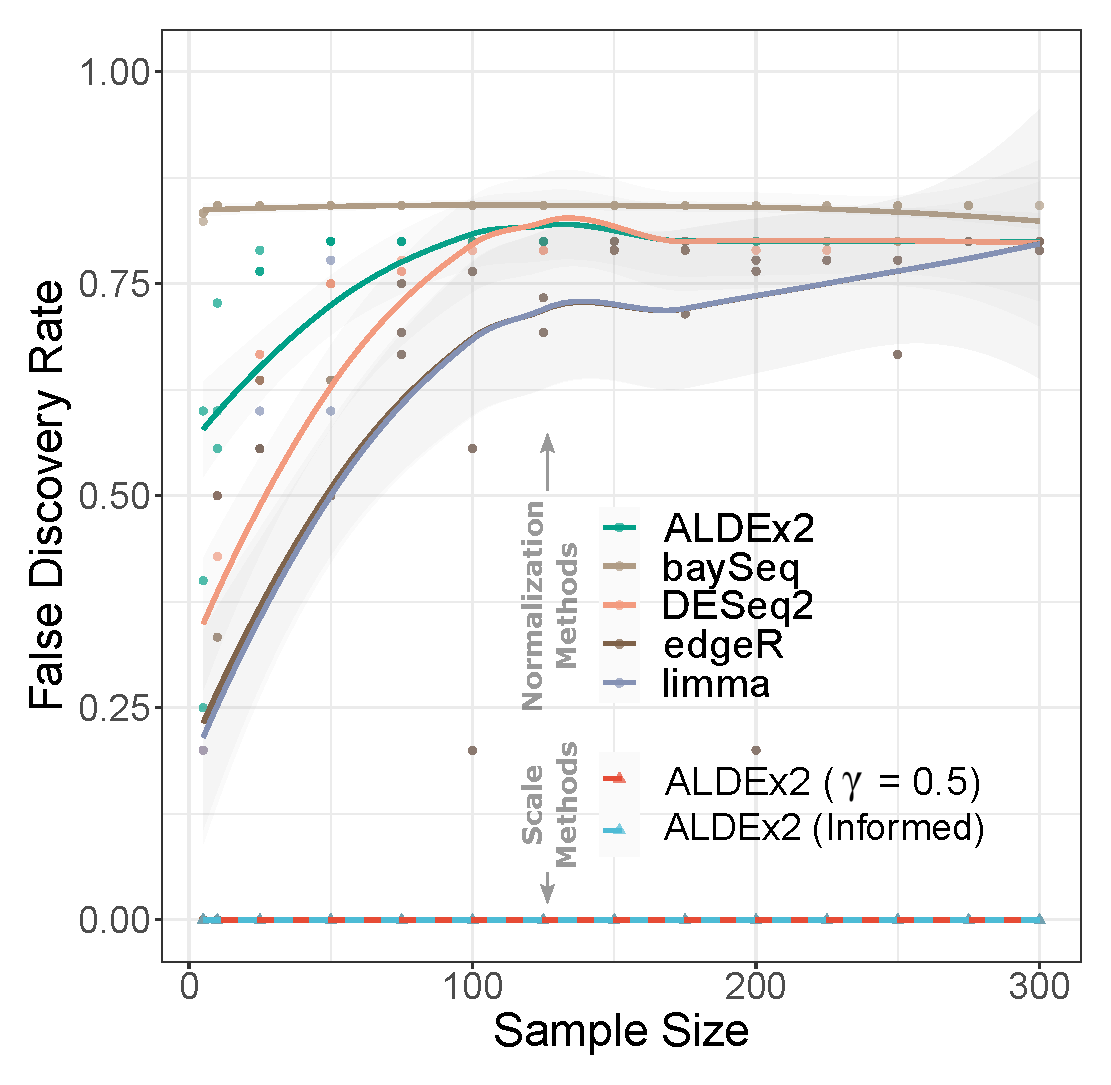
\includegraphics[width=3.25in]{figures/sim-res-samples.pdf}
\end{figure}
\end{frame}

\hypertarget{updated-aldex2-model}{%
\section{Updated ALDEx2 Model}\label{updated-aldex2-model}}

\begin{frame}{ALDEx2 as an SSRV}
\protect\hypertarget{aldex2-as-an-ssrv-1}{}
\textcolor{gray}{\textbf{Step 1: Model Sampling Uncertainty}}
\textcolor{gray}{\begin{align*}
\mathbf{Y}_{\cdot n} &\sim \text{Multinomial}(\mathbf{W}_{\cdot n}^\parallel)\\
\mathbf{W}_{\cdot n}^\parallel &\sim \text{Dirichlet}(\alpha)
\end{align*}}

\textbf{Step 2: Draw Samples from a Scale Model} \begin{align*}
\log W_{n}^\perp &\sim Q\\
\log \mathbf{W}_{\cdot n} &= \log \mathbf{W}_{\cdot n}^\parallel + \log W_{n}^\perp
\end{align*}

\textcolor{gray}{\textbf{Step 3: Calculate LFCs and Test if Different from Zero.}}
\textcolor{gray}{\begin{equation*}
\theta_d = \text{mean}_{\text{case}}(\log \mathbf{W}_{dn}) - \text{mean}_{\text{control}}(\log \mathbf{W}_{dn})
  \end{equation*}}
\end{frame}

\begin{frame}{Intro to Scale Models}
\protect\hypertarget{intro-to-scale-models}{}
There are no restrictions on what scale models can be, although there
are some helpful options:

\vspace{.125in}

\begin{enumerate}
\tightlist
\item
  Based on normalizations. \textcolor{gray}{(Stochastic normalizations)}
\item
  Based on biological knowledge.
\item
  Based on outside measurements.
\end{enumerate}
\end{frame}

\begin{frame}{Scale Models based on Biological Knowledge}
\protect\hypertarget{scale-models-based-on-biological-knowledge}{}
What do past studies or biological mechanisms tell about the scale of
the system?

\vspace{.1in}

\pause

\begin{itemize}
\tightlist
\item
  A past study showed that a certain disease (e.g., Crohn's disease)
  leads to lower microbial load in the gut.
\end{itemize}

\pause

\begin{align*}
\log W^\perp_{\text{Healthy}} &\sim N(1, \gamma^2)\\
\log W^\perp_{\text{Crohn's}} &\sim N(0.7, \gamma^2)
\end{align*}
\end{frame}

\begin{frame}{Scale Models based on Outside Measurements}
\protect\hypertarget{scale-models-based-on-outside-measurements}{}
How can outside measurements be used to quantify scale?

\vspace{.1in}

\pause

\begin{enumerate}
\item
  These measurements can be used \emph{if} they relate to your scale of
  interest.
\item
  Examples include flow cytometry, qPCR, etc.
\item
  Scale models can incorporate measurement uncertainty.
\end{enumerate}

\pause

\begin{equation*}
\log W^\perp_{n} \sim N(\log \mu_{FC,n}, \sigma^{2}_{FC,n})
\end{equation*}
\end{frame}

\hypertarget{changes-to-the-aldex2-interface}{%
\section{Changes to the ALDEx2
Interface}\label{changes-to-the-aldex2-interface}}

\begin{frame}[fragile]{Including scale}
\protect\hypertarget{including-scale}{}
\textbf{The new ALDEx2 model removes normalizations in lieu of scale
models.}

\vspace{.25in}

\pause

Major updates:

\begin{enumerate}
\tightlist
\item
  A new argument \texttt{gamma} which makes it easy to incorporate scale
  uncertainty (\texttt{aldex} and \texttt{aldex.clr} functions).
\end{enumerate}

\begin{itemize}
\tightlist
\item
  \texttt{gamma} can either be a single numeric or a matrix.

  \begin{enumerate}
  \tightlist
  \item
    Single numeric: controls the noise on the default scale model.
  \item
    Matrix: A \(N \times S\) matrix of samples of \(W^\perp\).
  \end{enumerate}
\end{itemize}

\begin{enumerate}
\setcounter{enumi}{1}
\tightlist
\item
  A new function \texttt{aldex.senAnalysis} to see how analysis results
  change as a function of scale uncertainty.
\end{enumerate}
\end{frame}

\begin{frame}{Option 1: Default Scale Model}
\protect\hypertarget{option-1-default-scale-model}{}
The default scale model is based on errors in the CLR normalization.

\[\log \hat{W}_{n}^{\perp(s)} = - \mathrm{mean} \left(\log \hat{W}^{\parallel (s)}_{\cdot n}\right) + \Lambda^\perp x_{n}\]
\[\Lambda^\perp  \sim \ N(0, \gamma^2).\] \pause 

\begin{enumerate}
\tightlist
\item
  When \(\gamma = 0\), behavior matches the original ALDEx2 model.
\end{enumerate}

\pause

\begin{enumerate}
\setcounter{enumi}{1}
\tightlist
\item
  For any value of \(\gamma > 0\), it models potential error in the CLR
  assumption
  \textcolor{gray}{(false positives will decrease compared to the CLR normalization.)}
\end{enumerate}

\pause

\begin{enumerate}
\setcounter{enumi}{2}
\tightlist
\item
  It has a concrete interpretation to contextualize scale assumptions.
\end{enumerate}
\end{frame}

\begin{frame}{Interpreting the Default Scale Model}
\protect\hypertarget{interpreting-the-default-scale-model}{}
\begin{align*}
\theta^\perp_{\text{Default Scale}} &= \text{mean}_{\text{case}}(-\text{GM}( \mathbf{W}_{\cdot n}^\parallel)) - \text{mean}_{\text{control}}(-\text{GM}( \mathbf{W}_{\cdot n}^\parallel)) + \epsilon\\
&= \theta^\perp_{\text{CLR}} + \epsilon\\
\epsilon &\sim N(0, \gamma^2)
\end{align*}

\pause

The default scale model implies that:

\pause

\begin{itemize}
\tightlist
\item
  With 95\% certainty, the value of \(\theta^\perp\) is within
  \(\pm 2 \gamma\) of the value of \(\theta^\perp_{\text{CLR}}\).
\end{itemize}

\pause

\begin{itemize}
\tightlist
\item
  With 95\% certainty, the true difference in scales falls within the
  the range \(2^{\theta_{\text{CLR}}^\perp \pm 2 \gamma}\).
\end{itemize}
\end{frame}

\begin{frame}{Example: Interpreting the Default Scale Model}
\protect\hypertarget{example-interpreting-the-default-scale-model}{}
With 95\% certainty, the true difference in scales falls within the the
range \(2^{\theta_{\text{CLR}}^\perp \pm 2 \gamma}\).

\pause

\begin{itemize}
\tightlist
\item
  Suppose that we are performing differential abundance in a
  case/control study where \(\theta_{\text{CLR}} = 0.04\).
\end{itemize}

\pause

\begin{itemize}
\tightlist
\item
  Suppose we set \(\gamma = 0.5\).
\end{itemize}

\pause

\begin{itemize}
\tightlist
\item
  Then, this implies that, with 95\% certainty, we believe that the
  scale of the case condition is within a factor of
  \([2^{0.04 - 2 \times 0.5}, 2^{0.04+ 2 \times 0.5}] = [0.51,2.05]\) of
  the control condition.
\end{itemize}
\end{frame}

\begin{frame}[fragile]{Using the Default Scale Model}
\protect\hypertarget{using-the-default-scale-model}{}
\begin{Shaded}
\begin{Highlighting}[]
\DocumentationTok{\#\# Adding noise via the default scale model}
\NormalTok{mod.defaultScale }\OtherTok{\textless{}{-}} \FunctionTok{aldex}\NormalTok{(Y, conds, }\AttributeTok{gamma =} \FloatTok{0.5}\NormalTok{)}
\end{Highlighting}
\end{Shaded}
\end{frame}

\begin{frame}[fragile]{Option 2: More Complex Scale Models}
\protect\hypertarget{option-2-more-complex-scale-models}{}
Alternatively, can pass a matrix of scale samples to \texttt{gamma} so
long as:

\begin{enumerate}
\tightlist
\item
  The dimension is \(N \times S\).
\item
  They are samples of \(W^\perp\) not \(\log W^\perp\).
\end{enumerate}

\pause

Reasons to do this:

\begin{enumerate}
\item
  \textbf{Biological beliefs:} Scale is guided by the biological system
  or the researcher's prior beliefs.
\item
  \textbf{Outside Measurements:} These can be used in building a scale
  model \emph{if} they are informative on the scale of interest (e.g.,
  qPCR, flow cytometry).
\end{enumerate}
\end{frame}

\begin{frame}{Sensitivity Analyses}
\protect\hypertarget{sensitivity-analyses}{}
\begin{itemize}
\tightlist
\item
  Instead of picking \(\gamma\), why not test over a range instead?
\end{itemize}
\end{frame}

\begin{frame}{Sensitivity Analyses}
\protect\hypertarget{sensitivity-analyses-1}{}
\textcolor{gray}{\textbf{Step 1: Model Sampling Uncertainty}}
\textcolor{gray}{\begin{align*}
\mathbf{Y}_{\cdot n} &\sim \text{Multinomial}(\mathbf{W}_{\cdot n}^\parallel)\\
\mathbf{W}_{\cdot n}^\parallel &\sim \text{Dirichlet}(\alpha)
\end{align*}}

\textbf{Step 2: Draw Samples from a Scale Model} For a given \(\gamma\):
\begin{align*}
\log W_{n}^{\perp, \gamma} &= - \mathrm{mean} \left(\log \hat{W}^{\parallel (s)}_{\cdot n}\right) + \Lambda^\perp x_{n}\\
\Lambda^\perp  &\sim \ N(0, \gamma^2)\\
\log \mathbf{W^\gamma}_{\cdot n} &= \log \mathbf{W}_{\cdot n}^\parallel + \log W_{n}^{\perp, \gamma}
\end{align*}

\textcolor{gray}{\textbf{Step 3: Calculate LFCs and Test if Different from Zero.}}

\textbf{Step 4: Repeat for all desired values of $\gamma$.}
\end{frame}

\begin{frame}{Example: Sensitivity Analyses}
\protect\hypertarget{example-sensitivity-analyses}{}
\begin{figure}
  \centering
  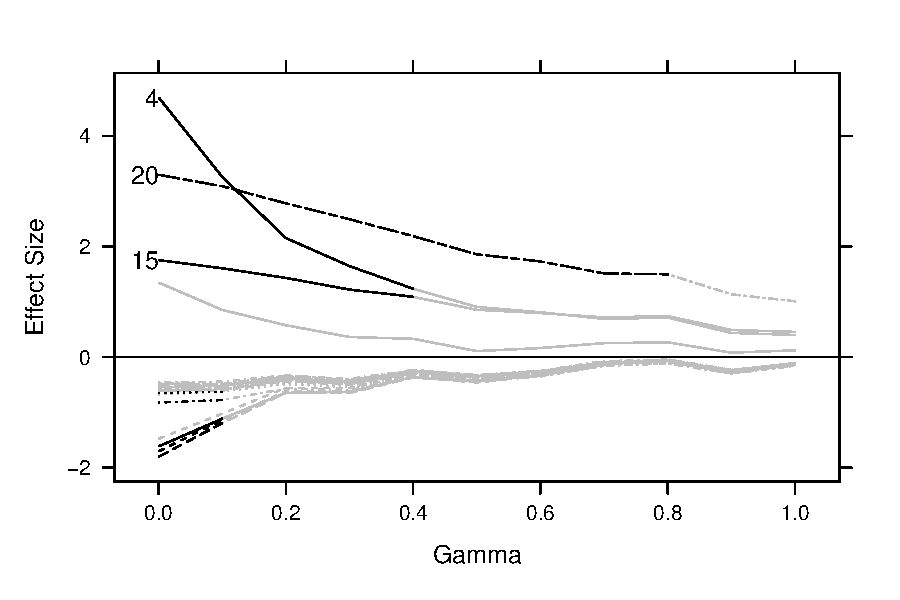
\includegraphics[width=4in]{figures/sim_gamma.pdf}
\end{figure}
\end{frame}

\hypertarget{data-examples}{%
\section{Data Examples}\label{data-examples}}

\begin{frame}{Simulation Study}
\protect\hypertarget{simulation-study}{}
Consider a simple study of the microbiome pre/post antibiotic
administration.

\begin{itemize}
\item
  \textbf{Research question:} Which taxa change in absolute abundance
  after taking an antibiotic?
\item
  100 study participants, 50 in each condition (pre/post antibiotics).
\item
  20 taxa total with 4 taxa truly changing
  \textcolor{gray}{(decreasing)}
\end{itemize}
\end{frame}

\begin{frame}{Data}
\protect\hypertarget{data}{}
\begin{figure}
  \centering
  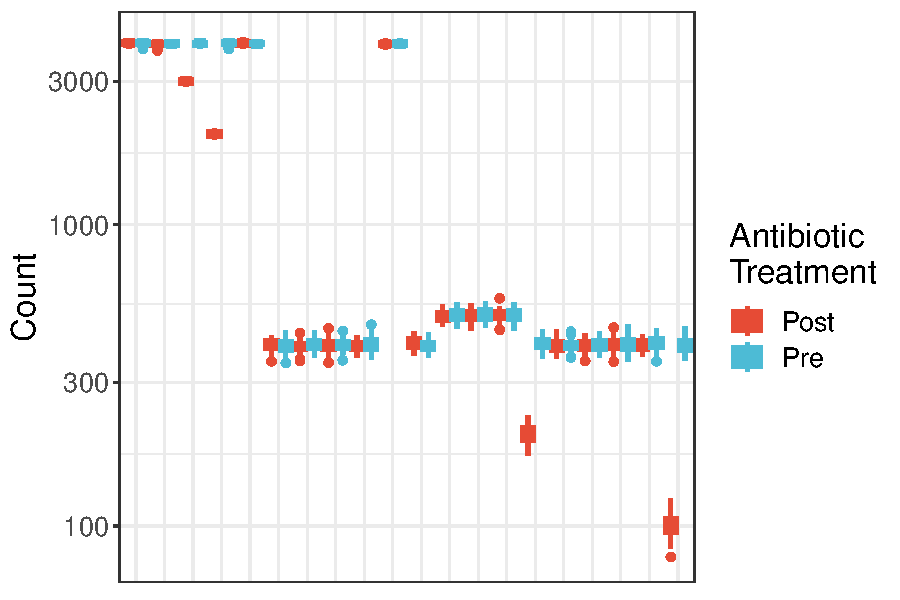
\includegraphics[width=4in]{figures/sim-data.pdf}
\end{figure}
\end{frame}

\begin{frame}[fragile]{Adding Scale is Easy}
\protect\hypertarget{adding-scale-is-easy}{}
\begin{Shaded}
\begin{Highlighting}[]
\DocumentationTok{\#\# Adding noise via the default scale model}
\NormalTok{mod.ss.high }\OtherTok{\textless{}{-}} \FunctionTok{aldex}\NormalTok{(Y, conds, }\AttributeTok{gamma =} \FloatTok{0.5}\NormalTok{)}
\end{Highlighting}
\end{Shaded}
\end{frame}

\begin{frame}[fragile]{Investigating Assumptions about Scale}
\protect\hypertarget{investigating-assumptions-about-scale}{}
\begin{Shaded}
\begin{Highlighting}[]
\DocumentationTok{\#\# Looking at the implied scale}
\NormalTok{clr }\OtherTok{\textless{}{-}} \FunctionTok{aldex.clr}\NormalTok{(Y, conds, }\AttributeTok{gamma =} \FloatTok{1e{-}3}\NormalTok{)}
\NormalTok{clr}\SpecialCharTok{@}\NormalTok{scaleSamps[}\DecValTok{1}\SpecialCharTok{:}\DecValTok{6}\NormalTok{, }\DecValTok{1}\SpecialCharTok{:}\DecValTok{4}\NormalTok{]}
\end{Highlighting}
\end{Shaded}

\begin{verbatim}
##          [,1]     [,2]     [,3]     [,4]
## [1,] 5.174279 5.124890 5.199780 5.175163
## [2,] 5.175705 5.144470 5.184953 5.167715
## [3,] 5.178751 5.171188 5.130795 5.100749
## [4,] 5.158594 5.195139 5.164371 5.145696
## [5,] 5.120674 5.175533 5.189581 5.171154
## [6,] 5.208741 5.273464 5.207085 5.162631
\end{verbatim}
\end{frame}

\begin{frame}{Investigating Assumptions about Scale, cont.}
\protect\hypertarget{investigating-assumptions-about-scale-cont.}{}
\begin{center}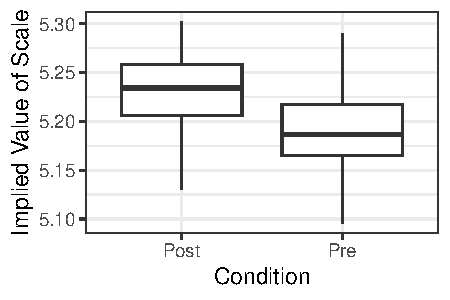
\includegraphics{slides_files/figure-beamer/unnamed-chunk-6-1} \end{center}
\end{frame}

\begin{frame}[fragile]{Scale Model based on Biology}
\protect\hypertarget{scale-model-based-on-biology}{}
\begin{Shaded}
\begin{Highlighting}[]
\DocumentationTok{\#\# Creating an informed model using biological reasoning}
\NormalTok{scales }\OtherTok{\textless{}{-}} \FunctionTok{c}\NormalTok{(}\FunctionTok{rep}\NormalTok{(}\DecValTok{1}\NormalTok{, }\DecValTok{50}\NormalTok{), }\FunctionTok{rep}\NormalTok{(}\FloatTok{0.9}\NormalTok{, }\DecValTok{50}\NormalTok{))}
\NormalTok{scale\_samps }\OtherTok{\textless{}{-}} \FunctionTok{aldex.makeScaleMatrix}\NormalTok{(}
  \AttributeTok{gamma =}\NormalTok{ .}\DecValTok{15}\NormalTok{,}
  \AttributeTok{mu =}\NormalTok{ scales,}
  \AttributeTok{conditions =}\NormalTok{ conds,}
  \AttributeTok{log =} \ConstantTok{FALSE}
\NormalTok{)}

\NormalTok{mod.know }\OtherTok{\textless{}{-}} \FunctionTok{aldex}\NormalTok{(Y, conds, }\AttributeTok{gamma =}\NormalTok{ scale\_samps)}
\end{Highlighting}
\end{Shaded}
\end{frame}

\begin{frame}[fragile]{Scale Model based on Outside Measurements}
\protect\hypertarget{scale-model-based-on-outside-measurements}{}
\begin{Shaded}
\begin{Highlighting}[]
\NormalTok{scale\_samps }\OtherTok{\textless{}{-}} \FunctionTok{matrix}\NormalTok{(}\ConstantTok{NA}\NormalTok{,}
  \AttributeTok{nrow =} \FunctionTok{nrow}\NormalTok{(flow\_data\_collapse),}
  \AttributeTok{ncol =} \DecValTok{128}
\NormalTok{)}

\ControlFlowTok{for}\NormalTok{ (i }\ControlFlowTok{in} \DecValTok{1}\SpecialCharTok{:}\FunctionTok{nrow}\NormalTok{(scale\_samps)) \{}
\NormalTok{  scale\_samps[i, ] }\OtherTok{\textless{}{-}} \FunctionTok{rnorm}\NormalTok{(}
    \AttributeTok{n =} \DecValTok{128}\NormalTok{,}
    \AttributeTok{mean =}\NormalTok{ flow\_data\_collapse}\SpecialCharTok{$}\NormalTok{mean[i],}
    \AttributeTok{sd =}\NormalTok{ flow\_data\_collapse}\SpecialCharTok{$}\NormalTok{stdev[i]}
\NormalTok{  )}
\NormalTok{\}}
\NormalTok{mod.flow }\OtherTok{\textless{}{-}} \FunctionTok{aldex}\NormalTok{(Y, conds, }\AttributeTok{gamma =}\NormalTok{ scale\_samps)}
\end{Highlighting}
\end{Shaded}
\end{frame}

\begin{frame}{Plotting Results}
\protect\hypertarget{plotting-results}{}
\begin{center}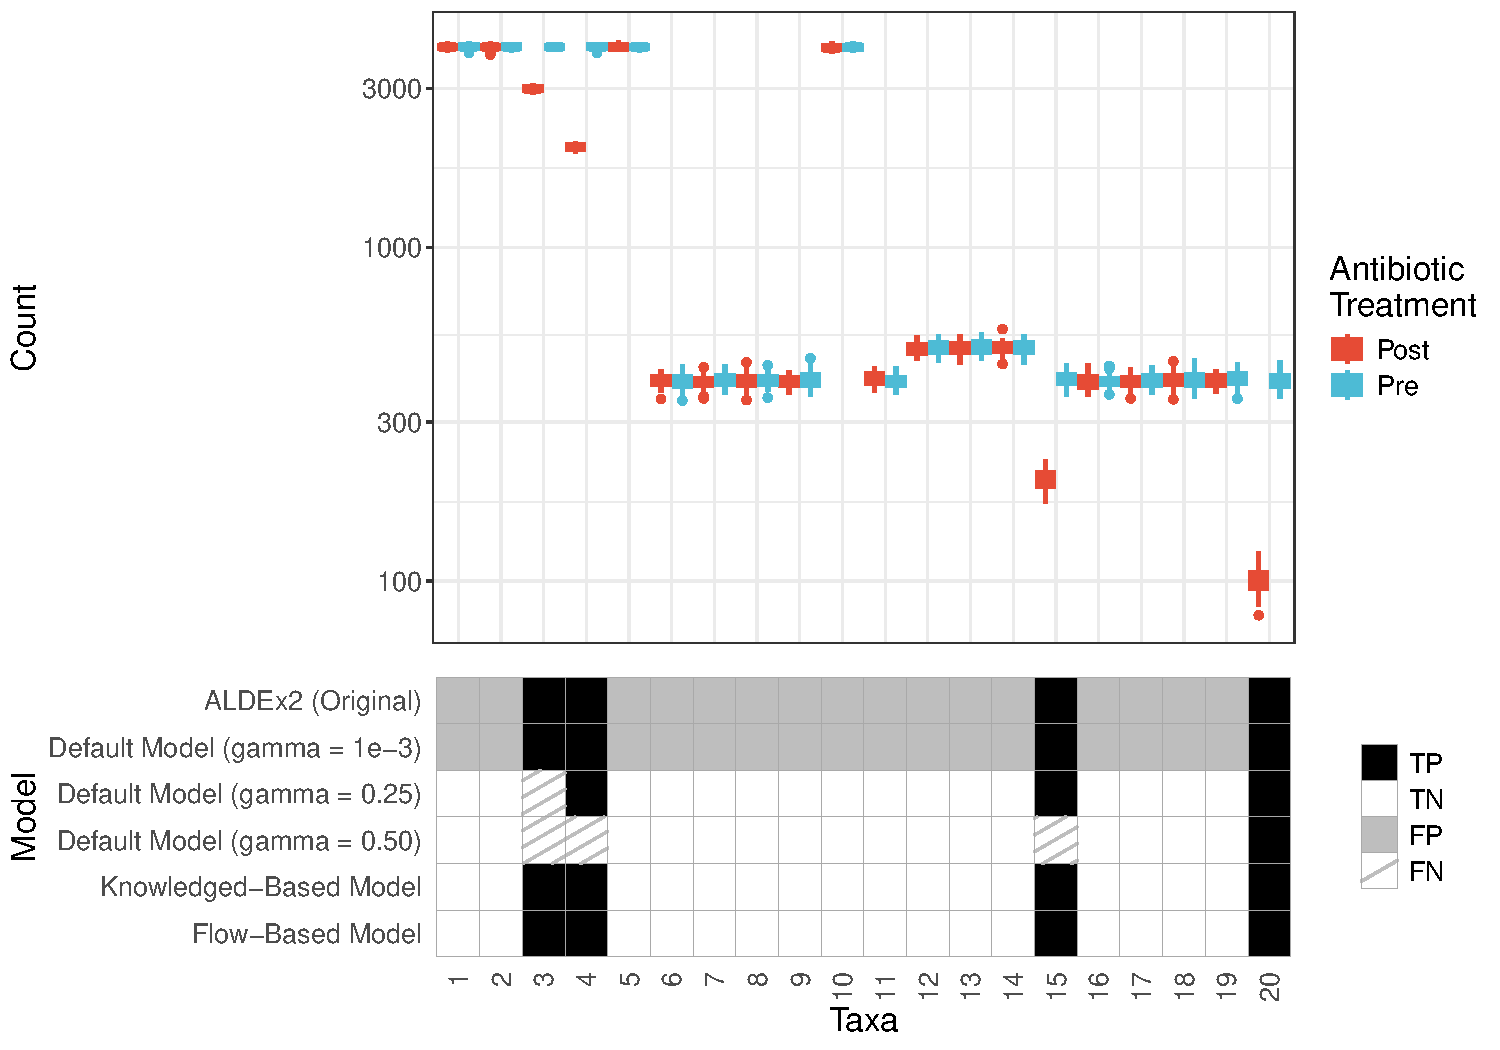
\includegraphics[width=0.95\linewidth]{slides_files/figure-beamer/unnamed-chunk-10-1} \end{center}
\end{frame}

\begin{frame}[fragile]{Sensitivity Analyses}
\protect\hypertarget{sensitivity-analyses-2}{}
\begin{Shaded}
\begin{Highlighting}[]
\DocumentationTok{\#\# First, specifying different values for the noise in the scale}
\NormalTok{gamma\_to\_test }\OtherTok{\textless{}{-}} \FunctionTok{c}\NormalTok{(}\FloatTok{1e{-}3}\NormalTok{, }\FunctionTok{seq}\NormalTok{(}\FloatTok{0.1}\NormalTok{, }\DecValTok{1}\NormalTok{, }\AttributeTok{by =}\NormalTok{ .}\DecValTok{1}\NormalTok{))}

\DocumentationTok{\#\# Run the CLR function}
\NormalTok{clr }\OtherTok{\textless{}{-}} \FunctionTok{aldex.clr}\NormalTok{(Y, conds)}

\DocumentationTok{\#\# Run sensitivity analysis function}
\NormalTok{sen\_res }\OtherTok{\textless{}{-}} \FunctionTok{aldex.senAnalysis}\NormalTok{(clr,}
  \AttributeTok{gamma =}\NormalTok{ gamma\_to\_test}
\NormalTok{)}
\FunctionTok{plotGamma}\NormalTok{(sen\_res,}
  \AttributeTok{thresh =}\NormalTok{ .}\DecValTok{1}\NormalTok{,}
  \AttributeTok{blackWhite =} \ConstantTok{TRUE}\NormalTok{, }\AttributeTok{taxa\_to\_label =} \DecValTok{3}
\NormalTok{)}
\end{Highlighting}
\end{Shaded}
\end{frame}

\begin{frame}{Sensitivity Analyses, cont.}
\protect\hypertarget{sensitivity-analyses-cont.}{}
\begin{figure}
  \centering
  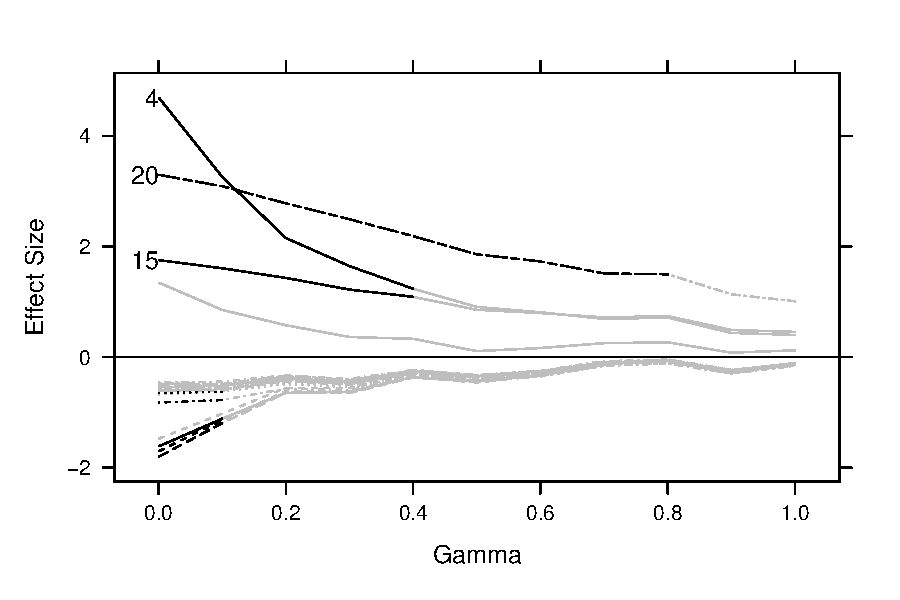
\includegraphics[width=4in]{figures/sim_gamma.pdf}
\end{figure}
\end{frame}

\begin{frame}{Real Example: Vandputte}
\protect\hypertarget{real-example-vandputte}{}
\begin{enumerate}
\item
  Comparison study of 29 Crohn's disease patients and 66 healthy
  controls.
\item
  For each patient, they sequenced the fecal sample and obtained flow
  cytometry measurements.
\item
  Proposed an approach that supplemented sequence count data with flow
  cytometry measurements.
\end{enumerate}
\end{frame}

\begin{frame}{Difference in Scale Implied by Flow Cytometry}
\protect\hypertarget{difference-in-scale-implied-by-flow-cytometry}{}
\begin{center}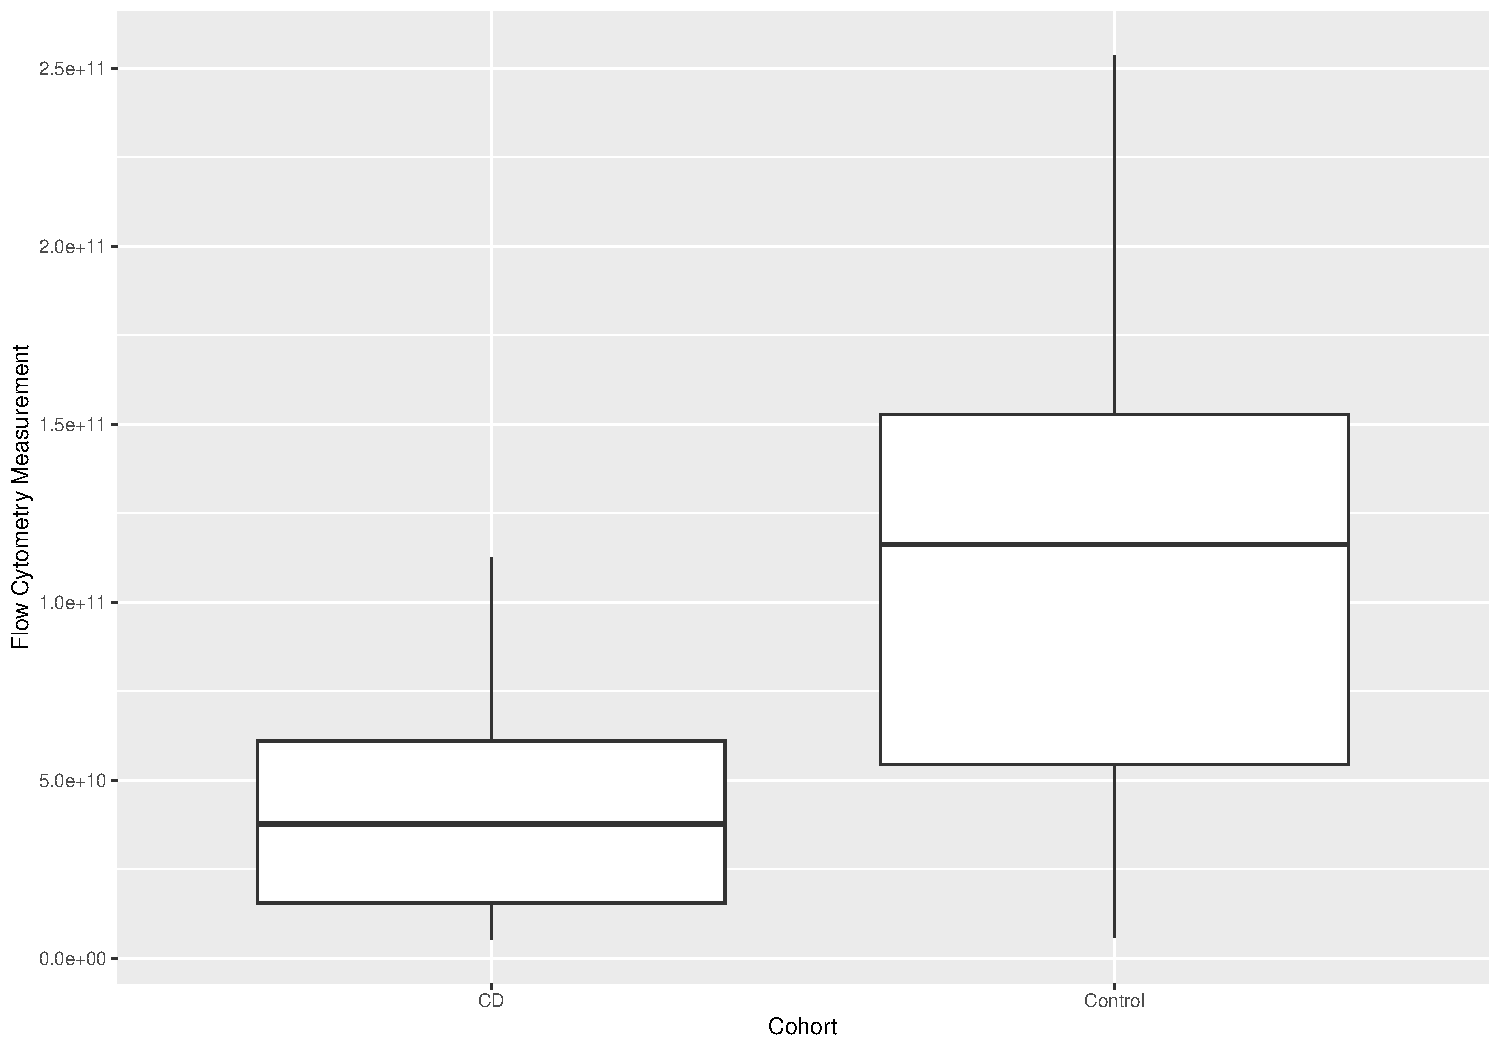
\includegraphics[width=0.95\linewidth]{slides_files/figure-beamer/unnamed-chunk-13-1} \end{center}
\end{frame}

\begin{frame}{Difference in Scale Implied by CLR}
\protect\hypertarget{difference-in-scale-implied-by-clr}{}
\begin{center}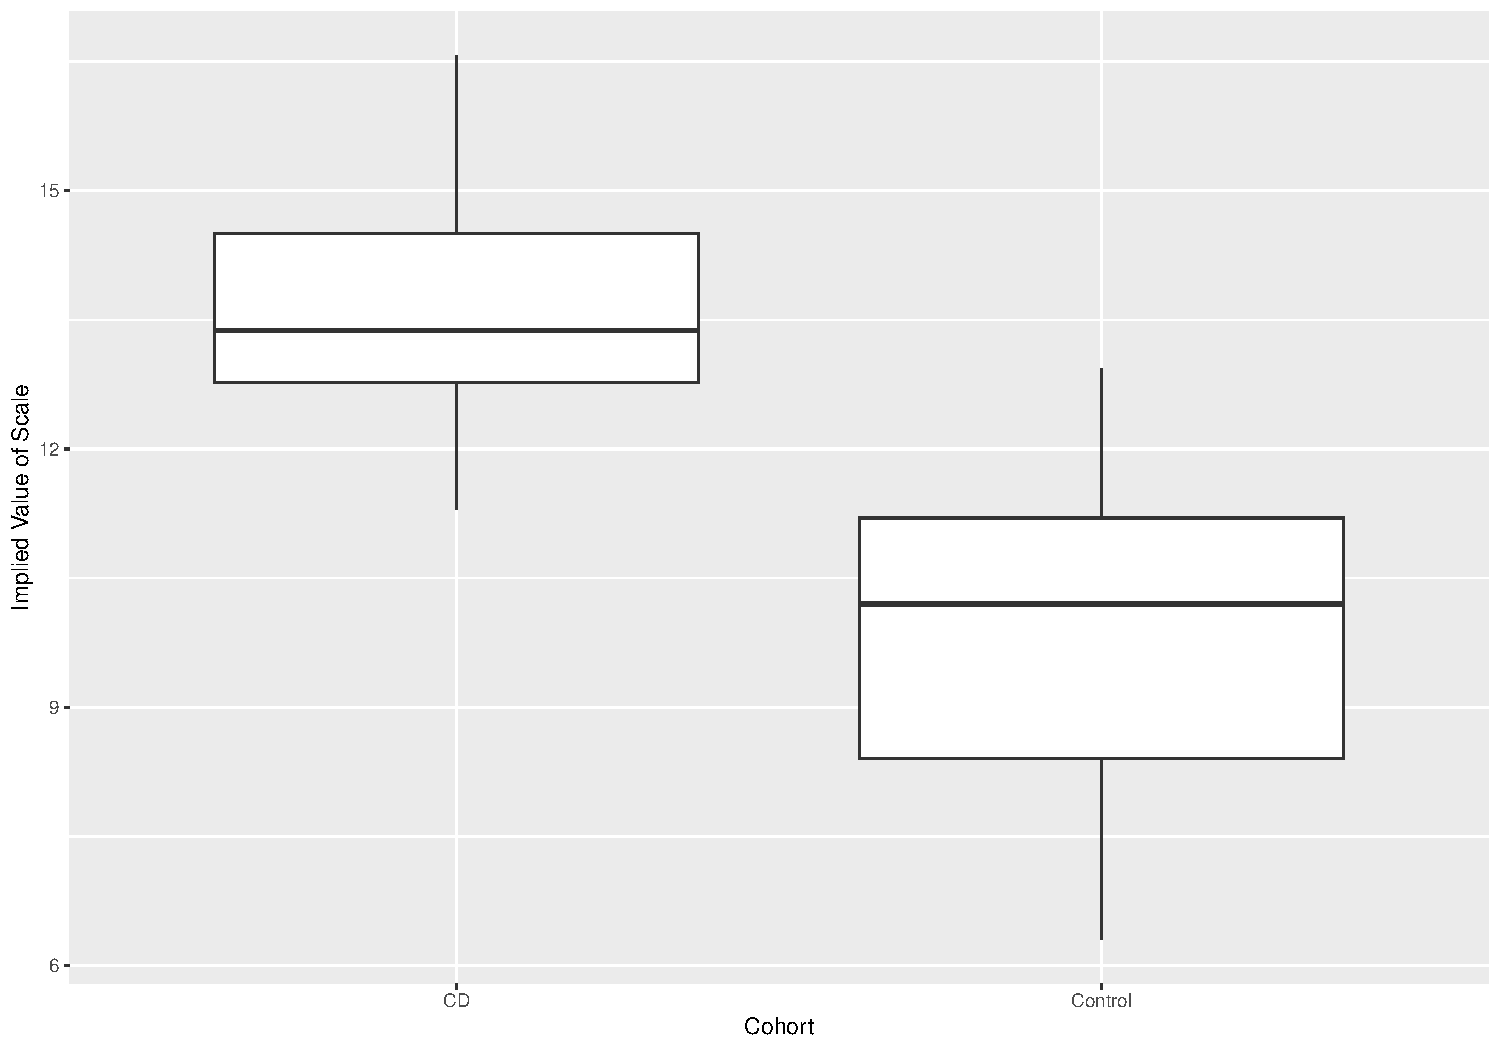
\includegraphics[width=0.95\linewidth]{slides_files/figure-beamer/unnamed-chunk-14-1} \end{center}
\end{frame}

\begin{frame}[fragile]{Creating a Gold Standard Model}
\protect\hypertarget{creating-a-gold-standard-model}{}
\begin{Shaded}
\begin{Highlighting}[]
\NormalTok{scale\_mean }\OtherTok{\textless{}{-}} \FunctionTok{log2}\NormalTok{(}\FunctionTok{sample\_data}\NormalTok{(phylo)}\SpecialCharTok{$}\NormalTok{CellCount)}
\NormalTok{scale\_var }\OtherTok{\textless{}{-}} \FunctionTok{rep}\NormalTok{(}\FloatTok{0.7}\NormalTok{, }\DecValTok{95}\NormalTok{)}

\NormalTok{scale\_samples }\OtherTok{\textless{}{-}} \FunctionTok{matrix}\NormalTok{(}\ConstantTok{NA}\NormalTok{, }\AttributeTok{nrow =} \DecValTok{95}\NormalTok{, }\AttributeTok{ncol =} \DecValTok{1000}\NormalTok{)}
\ControlFlowTok{for}\NormalTok{ (i }\ControlFlowTok{in} \DecValTok{1}\SpecialCharTok{:}\DecValTok{95}\NormalTok{) \{}
\NormalTok{  scale\_samples[i, ] }\OtherTok{\textless{}{-}} \DecValTok{2}\SpecialCharTok{\^{}}\FunctionTok{rnorm}\NormalTok{(}
    \DecValTok{1000}\NormalTok{,}
\NormalTok{    scale\_mean[i],}
\NormalTok{    scale\_var[i]}
\NormalTok{  )}
\NormalTok{\}}
\end{Highlighting}
\end{Shaded}
\end{frame}

\begin{frame}[fragile]{Creating an Informed Model}
\protect\hypertarget{creating-an-informed-model}{}
\begin{Shaded}
\begin{Highlighting}[]
\NormalTok{scale.cd }\OtherTok{\textless{}{-}} \DecValTok{2}\SpecialCharTok{\^{}}\FunctionTok{matrix}\NormalTok{(}\FunctionTok{rnorm}\NormalTok{(}\DecValTok{1000} \SpecialCharTok{*} \DecValTok{29}\NormalTok{,}
  \AttributeTok{mean =} \FunctionTok{log2}\NormalTok{(.}\DecValTok{7}\NormalTok{), }\AttributeTok{sd =}\NormalTok{ .}\DecValTok{125}
\NormalTok{), }\AttributeTok{nrow =} \DecValTok{29}\NormalTok{)}
\NormalTok{scale.control }\OtherTok{\textless{}{-}} \DecValTok{2}\SpecialCharTok{\^{}}\FunctionTok{matrix}\NormalTok{(}\FunctionTok{rnorm}\NormalTok{(}\DecValTok{1000} \SpecialCharTok{*} \DecValTok{66}\NormalTok{,}
  \AttributeTok{mean =} \FunctionTok{log2}\NormalTok{(}\DecValTok{1}\NormalTok{), }\AttributeTok{sd =}\NormalTok{ .}\DecValTok{125}
\NormalTok{), }\AttributeTok{nrow =} \DecValTok{66}\NormalTok{)}

\NormalTok{scale.informed }\OtherTok{\textless{}{-}} \FunctionTok{rbind}\NormalTok{(scale.cd, scale.control)}
\NormalTok{aldex\_informed }\OtherTok{\textless{}{-}} \FunctionTok{aldex}\NormalTok{(Y, X,}
  \AttributeTok{mc.samples =} \DecValTok{1000}\NormalTok{,}
  \AttributeTok{gamma =}\NormalTok{ scale.informed}
\NormalTok{)}
\end{Highlighting}
\end{Shaded}
\end{frame}

\begin{frame}{Comparing to Other Methods}
\protect\hypertarget{comparing-to-other-methods}{}
\begin{center}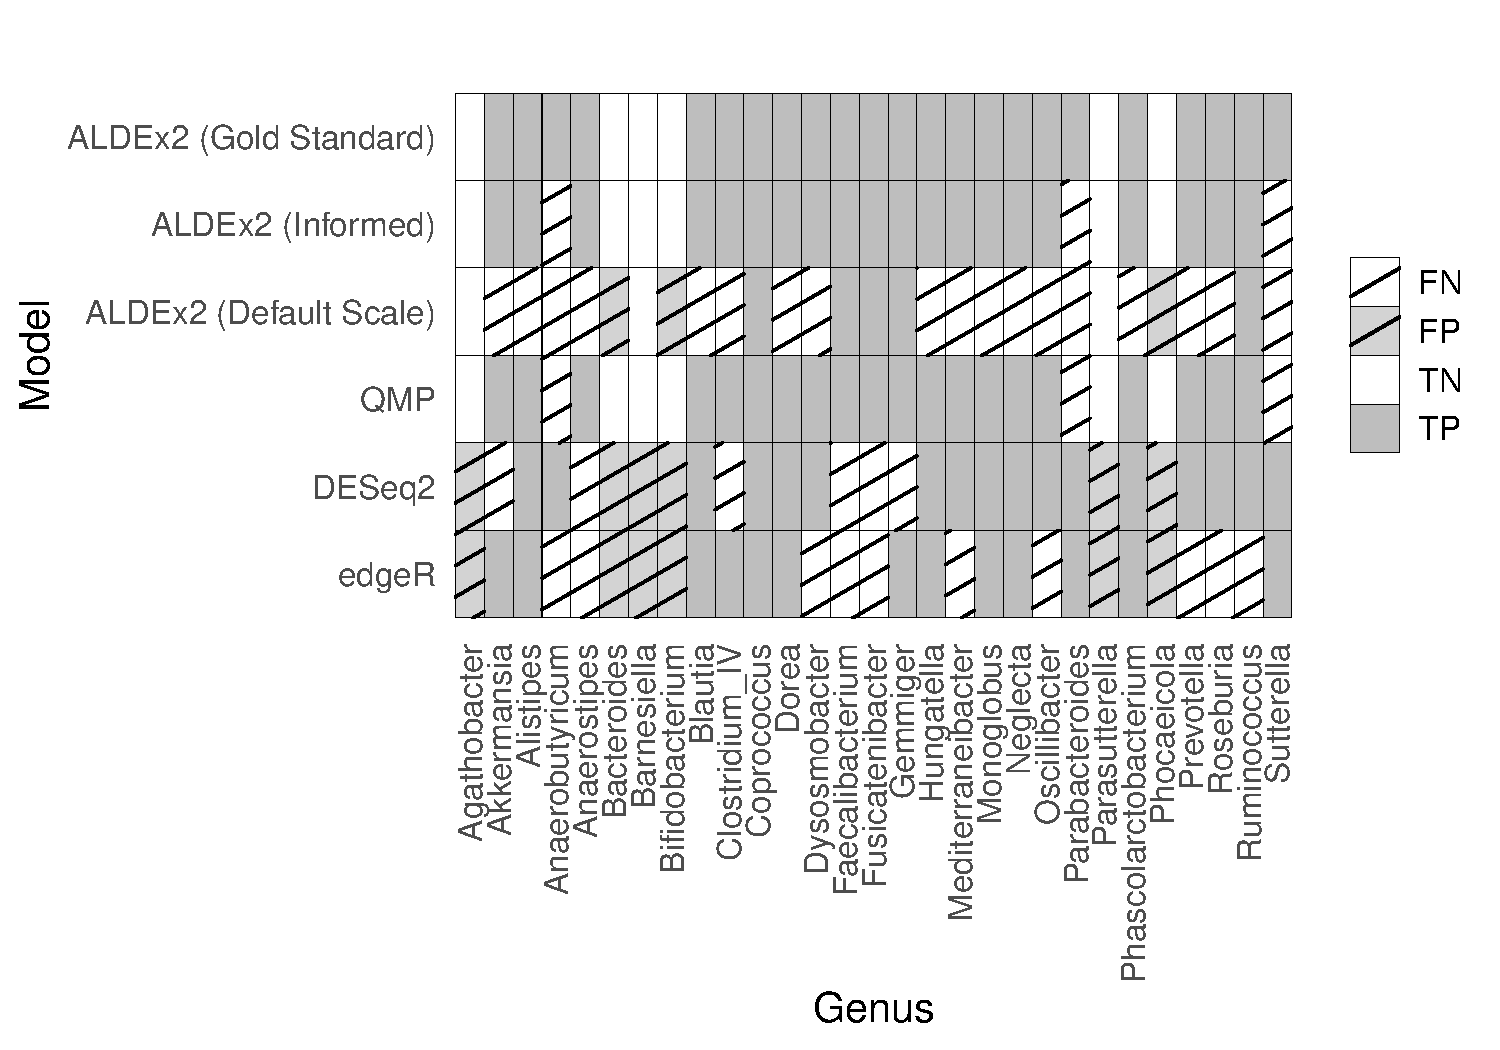
\includegraphics[width=0.95\linewidth]{slides_files/figure-beamer/unnamed-chunk-19-1} \end{center}
\end{frame}

\begin{frame}{Sensitivity Analyses}
\protect\hypertarget{sensitivity-analyses-3}{}
\begin{center}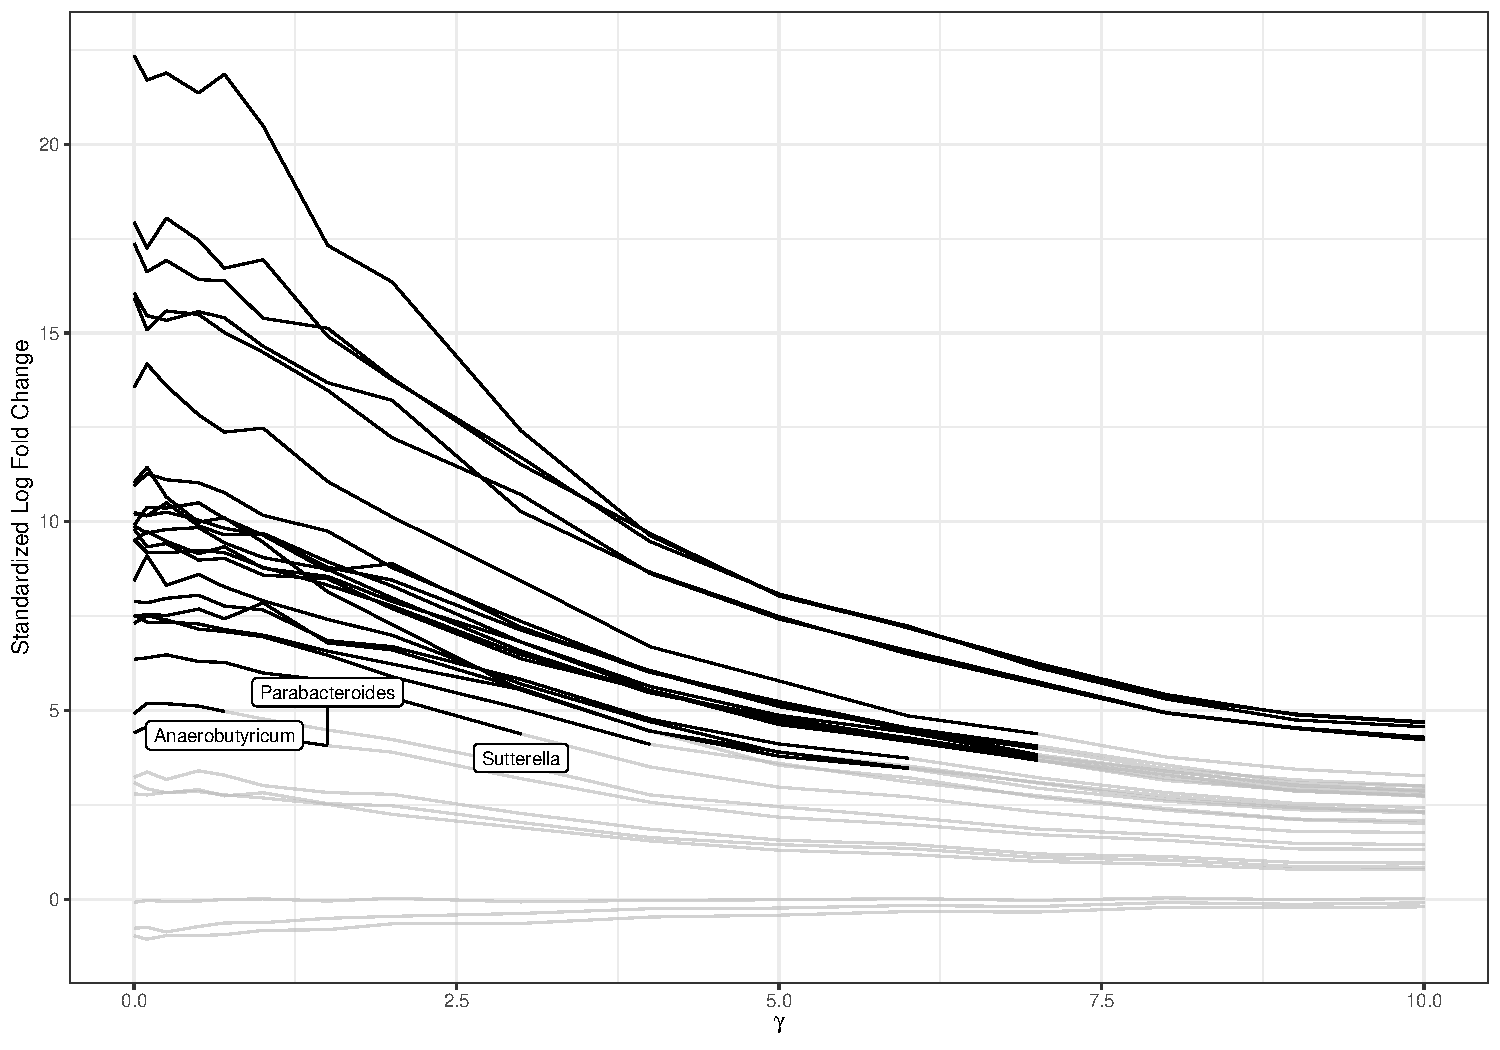
\includegraphics[width=0.95\linewidth]{slides_files/figure-beamer/unnamed-chunk-20-1} \end{center}
\end{frame}

\begin{frame}{References}
\protect\hypertarget{references}{}
\textbf{Scale Reliant Inference/Updates to ALDEx2:}

\begin{itemize}
\item
  Nixon, et. al.~(2023) ``Scale Reliant Inference.'' \emph{ArXiv
  Preprint 2201.03616}.
\item
  Gloor, Nixon, and Silverman. (2023) ``Scale is Not What You Think;
  Explicit Scale Simulation in ALDEx2.'' \emph{BioRXiv Preprint
  2023.10.21.563431}.
\item
  Nixon, Gloor, and Silverman. (2024) ``Beyond Normalizations:
  Incorporating Scale Uncertainty in ALDEx2.'' \emph{BioRXiv Preprint
  2024.04.01.587602}.
\item
  Fernandes et. al.~(2014). ``Unifying the analysis of high-throughput
  sequencing datasets: characterizing RNA-seq, 16S rRNA gene sequencing
  and selective growth experiments by compositional data analysis.''
  \emph{Microbiome}.
\end{itemize}
\end{frame}

\begin{frame}{References}
\protect\hypertarget{references-1}{}
\textbf{Data Sources:}

\begin{itemize}
\item
  McMurrough et. al.~(2014).''Control of catalytic efficiency by a
  co-evolving network of catalytic and non-catalytic residues.''
  \emph{PNAS}.
\item
  Vandputte et. al.~(2017). ``Quantitative microbiome profiling links
  gut community variation to microbial load.'' \emph{Nature}.
\end{itemize}
\end{frame}

\end{document}
